\documentclass[xcolor=dvipsnames,envcountsect]{beamer}


%----------▼▼▼▼▼ START PREAMBLE ▼▼▼▼▼----------

%-------- theme --------
\usetheme{Madrid}

%-------- color --------
\definecolor{crimsonred}{RGB}{0,153,0} % Green
\usecolortheme[named=crimsonred]{structure}
%-------- set color of 'example block' to crimson theme --------
\setbeamercolor{block body example}{bg=white}
\setbeamercolor{block title example}{fg=white, bg=green!50!black}

%-------- font --------
\setbeamerfont{structure}{family=\rmfamily,series=\bfseries}
\usefonttheme[stillsansseriftext]{structurebold}
\setbeamerfont{section in head/foot}{size=\tiny}

%-------- misc structure --------
\useoutertheme[footline=authortitle,subsection=false]{miniframes}
\useinnertheme{rounded}
\addtobeamertemplate{block begin}{}{\justifying}
\newtheorem{remark}[theorem]{Remark}
\renewcommand{\indent}{\hspace*{2em}}
\setbeamertemplate{theorems}[numbered]
\setbeamertemplate{caption}[numbered]
\usepackage[justification=centering]{caption}
\renewcommand{\qedsymbol}{$\blacksquare$}

%-------- packages to be used -------
\usepackage{amsmath,amsfonts,amssymb,amscd,amsthm}
\usepackage{graphicx,xcolor,comment}
\usepackage{mathrsfs} 
\usepackage{multirow}
\usepackage{array}
\usepackage{hyperref}
\usepackage{multicol}
\usepackage{ragged2e}
\usepackage{caption}
\usepackage[spanish]{babel}
\usepackage{rotating}
\usepackage{enumerate}
\usepackage{tikz}
\usepackage{bm}
\usepackage{csquotes}
\usepackage{lipsum}


%-------- for bibliography -----------------
\usepackage{biblatex}
\setbeamertemplate{bibliography item}{\insertbiblabel}
\addbibresource{References.bib}
\setbeamertemplate{frametitle continuation}{\frametitle{\color{white}List of References}}

%--------  Backgound -------------------
\usebackgroundtemplate{%
	\tikz[overlay,remember picture] \node[opacity=0.02, at=(current page.center)] {
		
\includegraphics[height=4.5in,width=4.5in]{./Figures/LOGO CATIM.png}};
		}


%----------▲▲▲▲▲ PREAMBLE END ▲▲▲▲▲----------
%-----------------------------------------------

%---------START EDITING HERE---------------------
\title[Título del seminario]{Título del seminario}

\author [Nombre del expositor]{\textbf{Nombre del expositor}}

\institute[Universidad Autónoma de Nuevo León] {\emph{Asesor de tesis: }\textbf{Nombre del asesor de tesis}\\[1em]
	Universidad Autónoma de Nuevo León\\Facultad de Ingeniería Mecánica y Eléctrica\\Cuerpo Académico Tecnología e Innovación Mecatrónica\\[1em]

\includegraphics[scale=0.09]{./Figures/LOGO UANL-FIME.png}}

\date[Mes Día, Año]{\footnotesize \textbf{Mes Día, Año}}


%--------- START DOCUMENT ------------------
\begin{document}
	
\begin{frame}{\titlepage}\end{frame}
\begin{frame}{\frametitle{Presentation Outline}\tableofcontents}\end{frame}


%--------- INTRODUCTION ----------------------
\section{Introduction}
\begin{frame}
	\frametitle{Introduction}
		\justifying
        \lipsum[18]
\end{frame}

%---------- DEFINITION/PRELIMINARY ---------------------
\section{Working Definitions}
\begin{frame}
	\frametitle{Working Definitions}
    \begin{definition}\label{d19} A  set $M \subseteq E(G)$ is an \emph{edge dominating set of $G$} if every $u \in E(G) \backslash M$ is adjacent to some $v \in M$. The     \emph{edge domination number of $G$}, denoted by $\gamma_{e}(G)$, is the minimum cardinality of an edge dominating set of $G$. Any edge dominating set of $G$ with cardinality $\gamma_{e}(G)$ is referred to as a \emph{$\gamma_{e}$-set of $G$}.
    \end{definition}
\end{frame}

\begin{frame}
	\frametitle{Working Definitions (Cont'n)}
	\begin{example}
	\justifying
		\normalfont{The sets $M_{1}=\{a, c, f\}, M_{2}=\{d, h\}$, and $M_{3}=\{a, e, g, h\}$ are edge dominating sets of $G$ in Figure 1.5. Moreover, $M_{2}=\{d, h\}$ is a minimum edge dominating set of $G$. Thus, $\gamma_{e}(G)=\left|M_{2}\right|=2$.}
		\begin{figure}[ht]
			\centering
			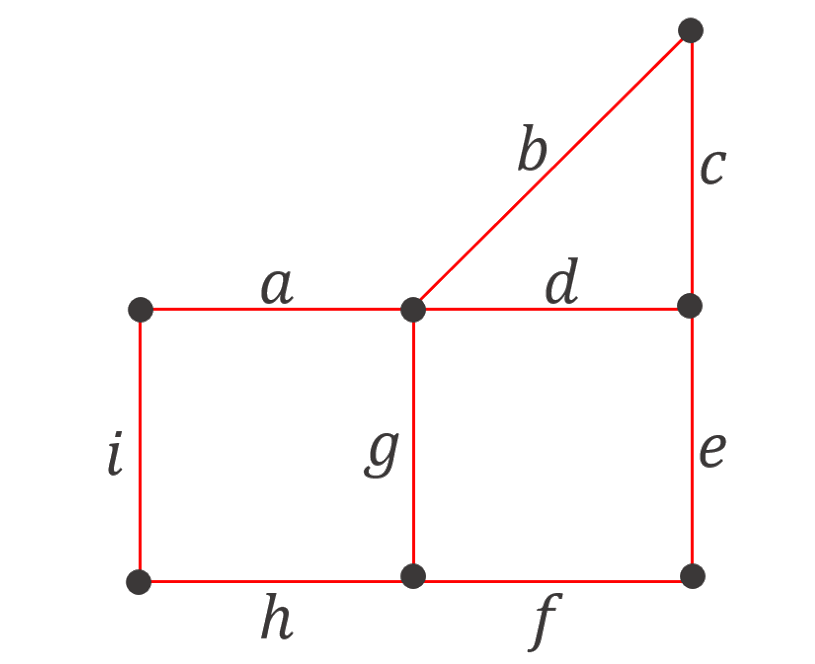
\includegraphics[width=0.35\textwidth]{./Figures/EDOM.png}
			\captionsetup{justification=centering}
			\caption{A graph $G$ with $\gamma_{e}(G)=2$.\label{edom}}
		\end{figure}
	\end{example}
\end{frame}


%----------- MAIN RESULTS ------------------------------
\section{Results}
\begin{frame}{Results}
		\begin{remark}\label{rem: 1}
		A set $S$ is an outer-connected edge dominating set of a graph $G$ if $S$ is an edge dominating set such that $H_{E(G) \backslash \mathrm{S}}$ does not have component isomorphic to $K_{2}$ or $S=E(G)$.
		\end{remark}
	\pause
	\indent To see this, consider graphs $G_{1}=P_{3}, G_{2}=P_{4}$, and $G_{3}=C_{8}$ in Figure \ref{3.1}.
	Then, $\gamma_{oce}(P_{3})=2, \gamma_{oce}(P_{4})=3$, and $\gamma_{o c e}(C_{8})=4$.
\end{frame}
\begin{frame}{Results (Cont'n)}
		\begin{figure}[ht]
		\centering
		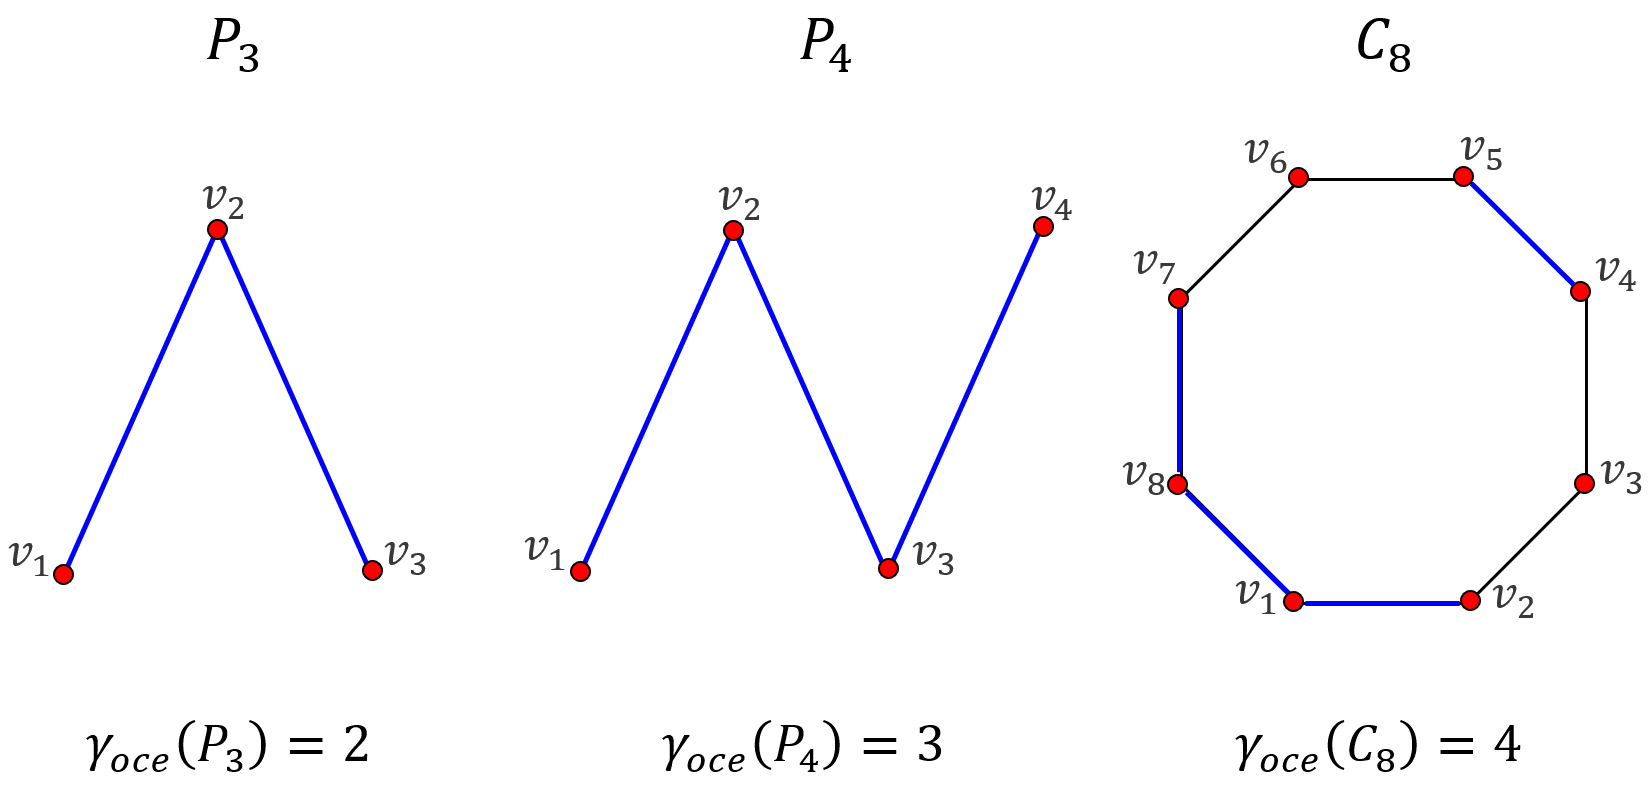
\includegraphics[width=0.9\textwidth]{./Figures/3.1.png}
		\caption{Graphs with $\gamma_{oce}(P_{3})=2, \gamma_{oce}(P_{4})=3$, and $\gamma_{oce}(C_{8})=4$.\label{3.1}}
		\end{figure} 
\end{frame}

%---------- RECOMMENDATIONS -----------------------------
\section{Recommendations}
\begin{frame}
	\frametitle{Recommendations}
	\justifying

    The following problems are suggested for further study:\\
    
    \lipsum[5]
    \nocite{ordaz2019collective,ordaz2021flock,ordaz2021autonomous}
\end{frame}


%----------- REFERENCES  -------------
%----------- No editing in references section ----------
%----------- edit only in References.bib ----------
\begin{frame}[allowframebreaks]
	\justifying
	\frametitle{List of References}
	\printbibliography
\end{frame}
	
%--------- THANK YOU Text --------------------------
\begin{frame}{\titlepage}\end{frame}

%\begin{frame}
%	\centering
%	\begin{block}
%		\scshape
%			\begin{center}
%				\Huge\emph{Thank You So Much!}
%			\end{center}
%	\end{block}
%\end{frame}
%----------------------------------------------------
\end{document}
